\section{Theorie}
\label{sec:Theorie}

\subsection{Fehlerrechnung}

Für die Fehlerfortpflanzung bei Gleichungen mit $N$ fehlerbehafteten Größen
wird jeweils die Formel zur Gaußschen Fehlerfortpflanzung

\begin{equation*}
  \sigma = \sqrt{\sum_{i=1}^{N}\biggl(\frac{\partial f(x_{\g{i}})}{\partial x_{\g{i}}}
  \sigma_{\g{i}}\biggr)^2}
\end{equation*}
mit der jeweiligen Funktion $f(x_{\g{i}})$, den Messgrößen $x_{\g{i}}$ und den
zugehörigen Fehlern $\sigma_i$ verwendet.
Zur Berechnung des arithmetischen Mittels von $N$ Messwerten wird jeweils die
Formel

\begin{equation*}
  \bar{x} = \frac{1}{N}\sum_{i=1}^{N}x_{\g{i}}
\end{equation*}
mit den Messwerten $x_i$ benutzt.
Die Standardabweichung des Mittelwerts wird jeweils mit der Gleichung

\begin{equation*}
  \bar{\sigma} = \sqrt{\frac{1}{N-1}\sum_{i=1}^{N}(x_{\g{i}} - \bar{x})^2}
\end{equation*}
mit den $N$ Messwerten $x_i$ berechnet.

\subsection{introduction}

Within this experiment we try to view the absorption spectrum of Rubidium with a diode laser.

\subsection{Functionality of a laser}
\label{sec:laser}

The scientific abbreviation \textbf{LASER} means "\textbf{L}ight \textbf{A}mplification by \textbf{S}timulated \textbf{E}mission of \textbf{R}adiation".
With the schematic functionality of a laser, presented in the following, a laser is able to emit
very monochromatic and highly coherent light. To realize a laser, four components are needed: a laser medium, a pump, a cooling system and a resonator.

However, the laser medium has to be a material, where a so called population inversion can be archieved by external excitation.
Therefore it is usefull, to consider a system with three energy levels like shown in illustration \ref{fig:threelevelsystem}.
\begin{figure}
  \centering
  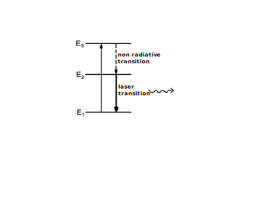
\includegraphics[height = 4.3cm]{Ordnername/threelevel_edit.pdf}
  \caption{Schematic plot of the three level system used in a laser medium \cite{threelevel} \textit{edited}.}
  \label{fig:threelevelsystem}
\end{figure}
The ground state is the most filled state at finite temperatur, like one can comprehend, when regarding the Boltzmann statistics.
With an external pumping the electrons from the ground state are excited to the instable third level and they immediatly transit to the second state
without emitting photons. The electrons from the second, more stable state fall back to the ground state at a smaller rate by spontaneous or stimulated emission.
With this configuration and a strong pumping an inversion population can be reached in contrast
to a two level system, where the maximum reached population in the second state is $\SI{50}{\percent}$.

There are several different possibilities, to excite the laser medium external, for instance thermal pumping,
electrical pumping, which is used in this experiment, or even chemical pumping.
In every case it is important, to cool the system well, because not the full energy, which is pumped into the system,
is converted to radiation. A non negligible part of the energy is transfered to phonons, so resulting in heat.
The cooling system will guarantee for a constant temperature of the laser medium, so that the thermal radiation stays constant
and the laser doesn't overheat.

However, the last but not least component of the laser is the resonator, see figure \ref{fig:lasersetup}.
The emitted photons of the laser medium radiate to the front and the backside of the laser can, where they are reflected. Of course the
front side mirror has to be partly reflecting, because there has to be an output beam. The reflected photons radiate back into the
laser medium and induce other radiation transitions with the same energy as the inducing photons. We emphasize, that this so called stimulated emission
is of great importance for the functionality of a laser, including the emission of monochromatic light. Beside this, another effect occurs:
Because of the mirrors on both sides the laser can forms a resonator for the beam. Only light modes with certain frequencies enjoy constructive interference
in the resonator and therefore their intensities are increased. The difference between the frequencies of two next neighbour modes is
called free spectral range and given by
\begin{align}
  \Delta \nu_\text{FSR} = \frac{\text{c}}{2 L n},
  \label{eqn:freespectralrange}
\end{align}
where $c$ is the speed of light, L is the length of the resonator and n is the refraction index of the laser medium.

\begin{figure}
  \centering
  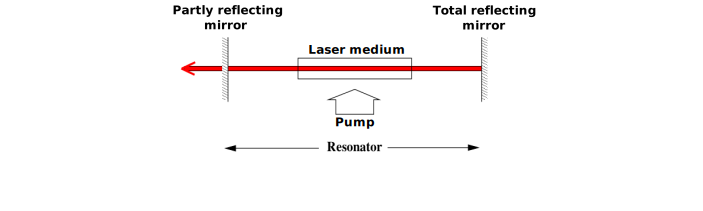
\includegraphics[height = 4.0cm]{Ordnername/lasersetup_edit.pdf}
  \caption{Setup of a laser in principle \cite{manual2} \textit{edited}.}
  \label{fig:lasersetup}
\end{figure}

With all the mentioned components of the laser setup one obtains an almost monochromatic and coherent laser beam.
To improve the laser with regard to its frequency width it is e.g. possible to build an external cavity with a diffraction
grating. We will treat this later both in theory and in experiment.

The main property of a diode laser is, that it contains a semiconductor medium and an electrical current pump, forming a diode.
Thus we present a short description of semiconductors, doping of them and the funcionality of a diode in the following sections.

\subsection{Semiconductors and doping}

A semiconductor is a material with two main properties: it conducts weaker than a metall, but stronger than an insulator and
its conductivity rises with the temperature. The illustrative reason for the enumerated things is, that the Fermi energy of
those materials is located inside a narrow band gap of the band structure. That means, that at zero temperature the valence band of a semiconductor is
filled, while the conducting band is empty, so no current can occur. At higher temperatures thermal excitations let the electrons overcome
the band gap, so that the conductivity increases.

Doping a semiconductor means placing impurities into it to change its conductivity substantial.
One distinguishes between doping with donor materials and doping with acceptor materials.
In the first case the impurity provides an additional electron, which is energetically by far closer to the
conductive band than the valence band. The consequence is, that the conductivity increases, because
the additional electrons only need to overcome a smaller band gap. In the second case the impurity
provides a hole, which lies energetically near to the valence band. This hole can be occupied by an electron
with much less energy than in the non doped case, so that the conductivity again rises.
Both concepts are illustrated in figures \ref{fig:donor} and \ref{fig:acceptor}.

\begin{figure}
  \centering
  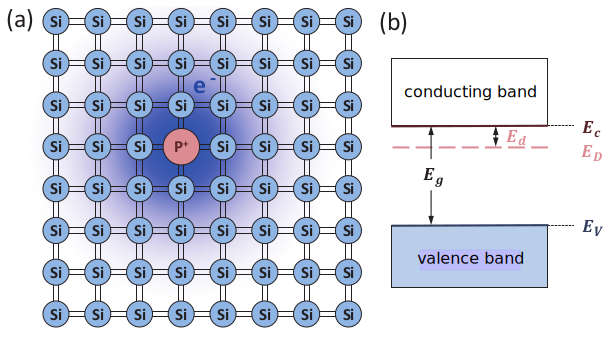
\includegraphics[height=5cm]{Ordnername/donor_edit.pdf}
  \caption{(a) Illustration of the grid of n-doped silicon. The phosphor impurity serves as an electron donor.
  (b) Schematic depiction of the band structure of a n-doped semiconductor \cite{semiconductors} \textit{edited}.}
  \label{fig:donor}
\end{figure}

\begin{figure}
  \centering
  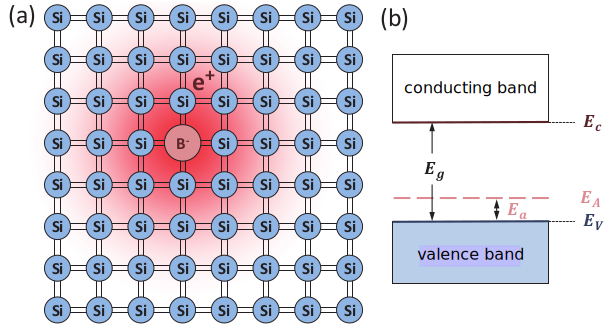
\includegraphics[height=5cm]{Ordnername/acceptor_edit.pdf}
  \caption{(a) Illustration of the grid of p-doped silicon. The boron impurity serves as an electron acceptor.
  (b) Schematic depiction of the band structure of a p-doped semiconductor \cite{semiconductors} \textit{edited}.}
  \label{fig:acceptor}
\end{figure}

\subsection{Funcionality of a diode}

Basically a diode consists of a semiconductor material, which is p-doped on one side and n-doped on the other side.
Without any external influences some of the almost not bounded electrons from the n-doped side will recombine, among emission of a photon,
with some holes from the p-doped side, caused by diffusion. The result is firstly a transition zone between the two doped sides, where
no free charge carriers remain, and secondly an electric field, which acts against the progress of recombination,
because it accelerates electrons from the p-doped side to the n-doped side. After a short time the system arrives at an equilibrium state,
where the diffusion current and the counter field current vanish. The width of the so called depletion zone at this point
depends on the doping densities and the diffusion potential.

However, if one attaches a power supply to the presented configuration, meaning to the diode, there are two relevant cases to consider:
In the first case the plus terminal is connected to the n-doped side, while the minus terminal is connected to the
p-doped side. The consequence is, that the doped semiconductor loses its conductivity, because the depletion layer width
increases as the remaining free charge carriers are pulled out by the power supply. One calls this configuration of the diode
the reverse or blocking direction. The second case includes connecting the poles the other way round, so that of course
the depletion layer width decreases and the conductivity rises. This setting is called the forward or passing direction of the diode.
As a conclusion of this section the current-voltage characteristic of the diode is presented in figure \ref{fig:currvolt}

\begin{figure}
  \centering
  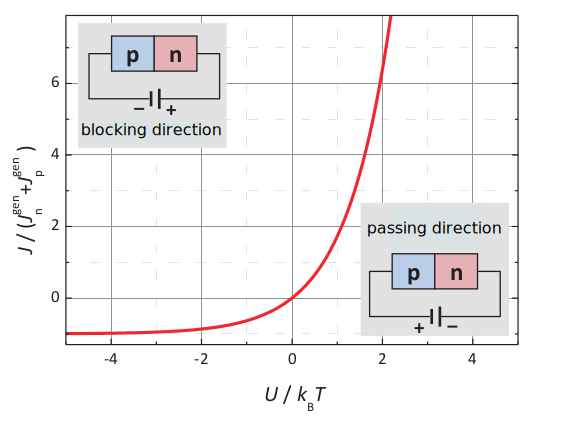
\includegraphics[height=6cm]{Ordnername/currvolt_edit.pdf}
  \caption{Current-voltage characteristic of the diode \cite{semiconductors} \textit{edited}.}
  \label{fig:currvolt}
\end{figure}

\subsection{Functionality of a diode laser}

To realize a diode laser, one has to operate with the diode in forward direction.
Electrons from the narrow depletion zone are pulled to the plus terminal, while
holes are pulled to the minus terminal. Because of diffusion, electrons and holes from the doped sides
recombine again in the depletion zone, while emitting a photon. Due to this, the depletion zone is
also called active layer. Its width stays constant within the permanent repetition of the enumerated
processes. So as a result of the pn-transition and the external electrical pumping one has a diode
with a light emitting active layer.

Because the active layer has a larger index of refraction than the surrounding layers, the emitted light is confined
and expands only within a tiny channel. To realize the resonator mentioned in section \ref{sec:laser} the front
and back facets of the semiconductor are cleaved to act as cavity mirrors. If the pump current lies under a
certain threshold, the stimulated gain is lower than the optical losses and the output of the diode laser is
comparable to that of a LED. Above this threshold the stimulated emission causes a population inversion and therefore
a strong light amplification. The intensity of the resulting coherent laser beam increases linearly with the current.

However, this is not the full necessary theoretical part of this experiment, because two problems occur:
The linewidth of the output beam is around $\Delta \nu \approx \SI{50}{\mega\hertz}$, so larger than the atomic transitions
of rubidium $\Delta \nu_\text{Rub} \approx \SI{5}{\mega\hertz}$ and the diode laser is very sensitive to optical feedback.
In the next section an optical instrument, which solves those problems, is presented.

\subsection{Optimizing the laser beam}

A possible solution of the enumerated problems in the last section is presented in figure \ref{fig:diffraction}.
After the output beam is collimated by a lens it hits a diffraction grating. With this optical tool, the optical
feedback is not deactivated, but controlled. Most of the light, however, is reflected by the diffraction grating,
but around $\SI{15}{\percent}$ strays back into the diode. So the grating and the back facet of the diode form
an external cavity for the laser beam. The consequences of this are explained later.

\begin{figure}
  \centering
  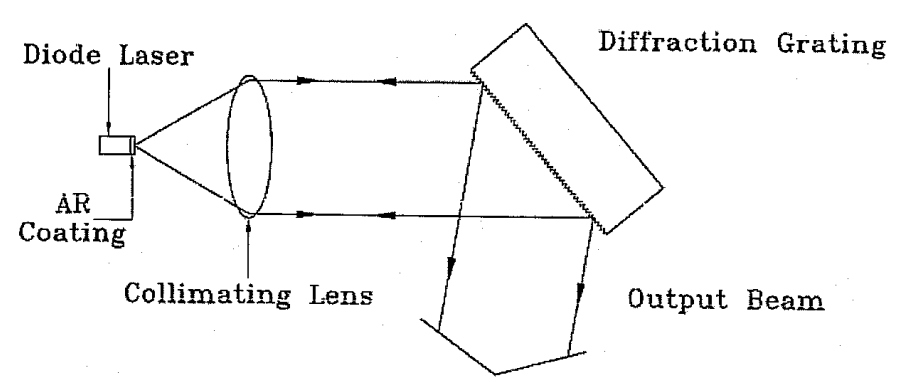
\includegraphics[height=5cm]{Ordnername/diffraction_edit.pdf}
  \caption{Setup of the diode laser with an external diffraction grating \cite{manual} \textit{edited}.}
  \label{fig:diffraction}
\end{figure}

Considering the total construction one has four different contributions to the optical gain of the laser:
the medium gain, the internal cavity, the grating feedback and the external cavity.
In figure \ref{fig:optgain} this is illustrated. Theoretically the laser will lase in the mode with the
highest net gain, because this mode amplifies itself the most via stimulated emission. In practice more
modes can occur at once and the output frequency can vary chaotically. One task in this experiment is to
estimate parameter configurations to get a single mode output through adjusting.

\begin{figure}
  \centering
  \includegraphics[height=7cm]{Ordnername/optgain.png}
  \caption{Schematic trend of the net gain for the four contributions \cite{manual}.}
  \label{fig:optgain}
\end{figure}

%One obtains that the wavelength increases almost linearly with the temperature.
The position of the maximum of the broad medium gain peak depends on the temperature of the laser.
After adjusting the temperature and therefore the wavelength to the required value, the medium gain can be neglected, because
of its broad peak.

Like mentioned before, the diode can forms an internal resonator or optical cavity, where frequently, as shown in equation
\eqref{eqn:freespectralrange}, certain wavelengths are amplified. The laser will tend to lase in those modes,
because the net gain is at the maximum. One can affect the wavelength by directly increasing the temperature of the
laser head, which is impractical, because it requires some time, or better by raising the current. The latter
increases firstly the temperature almost instantaneous and secondly the carrier concentration inside the active layer.



%This entails, that the output light





%linewidth



%780nanometer medium gain einstellen !



% laser daten -> free spectral range output power linewidth
%citation!!!!
